In order to perform the calibration of the quark-/gluon-jet tagger, it is requisite to establish two distinct subsamples. One subsample should be predominantly composed of quark-jets, called quark-enriched sample, while the other should predominantly consist of gluon-jets, as gluon-enriched sample. These subsamples are gained from the dijet events. This section describes the reconstruction and selection of jet objects used in this calibration, as well as the approach to construct quark- and gluon-enriched subsamples.

\subsubsection{Physics object definition}
\label{subsec:obj}

The PFlow jets that are reconstructed with the \antikt~algorithm with a radius parameter $R$ set to 0.4. An overall jet energy calibration described in section~\ref{sec:4.2} has been done to rectify residual detector effects and pile-up. In order to ensure a good quality jet, an event-based jet cleaning with standard loose cut is applied to reject events with flawed leading or subleading jet.

Tracks that reconstructed~\cite{ATLAS:2017kyn} from the ID are required to have \pt~> 500 MeV, and within the ID range \abseta < 2.5. Additional criteria such as primary vertex are required to ensure selected tracks originating from the collision and prevent the mis-reconstructed tracks from pile-up hits in the detector. The alignment of tracks with calorimeter-based jets is executed through the application of the ghost-association technique. This entails a repetition of the jet clustering procedure augmented by the inclusion of 'ghost' representations of registered tracks~\cite{CACCIARI2008119}. These ghost tracks share the same direction as their actual counterparts but possess an infinitesimally small \pt, thereby ensuring that they do not induce any alterations to the intrinsic characteristics of the calorimeter-based jets. A criterion for track-jet correspondence is established: a given track is associated to a jet if its corresponding ghost track is contained in the jet after reclustering.


Jet reconstructed from the simulated MC is known as "truth jets"~\cite{ATLAS:2020cli}, with the same \antikt $R=0.4$ algorithm as PFlow jets. Geometric correspondence between truth jets and PFlow jets is established via angular proximity, adhering to the criterion $\Delta R < 0.4$. Each truth jet is bestowed with a flavour label, referred to as a truth label~\cite{Aad_2014,ATL-PHYS-PUB-2017-009}. The truth flavour label attributed to a jet is defined by the flavour of the highest-energy parton situated within a cone of size $\Delta R < 0.4$ around the jet's axis, prior to the process of hadronisation in the parton shower. Following this definition, jets arising from the splintering of gluons into $b$- or $c$-quark pairs are labelled as heavy flavour jets. These heavy flavour jets are often identifiable by the long-lived or leptonically decaying hadrons. Therefore, no distinct discriminant tailored for heavy-flavour quarks is investigated within the current framework~\cite{CDF:2008ixu,ATLAS:2013uet}. Jets will be unlabelled if there is no corresponding truth parton with \pt $>$ 1 GeV is found within the cone surrounding the truth jet. These instances of unlabelled jets commonly emerge as a consequence of pile-up effects, and less than 1\% of the dataset used. They are thus ignored~\cite{ATLAS:2012mwf}.
 
 
  %through the following procedure: first, they are matched to the highest energy $b$-quark parton within $R$ = 0.3 of the truth jet axis. If one is found, the jet is labelled as a truth $b$-jet. If no $b$-quark parton is found, the procedure is repeated with $c$-quark partons. Both the $b$- and $c$-quark partons must have a \pt greater than 5 GeV. If no $c$-quark parton is found, then the highest energy light quark or gluon parton within a cone of R = 0.4 is used to assign the jet either a light quark or gluon label. Under this definition jets which originate from gluons splitting into $b$ or $c$-quark pairs will be labelled as heavy flavour jets. Because they are a small fraction of the overall event sample, any difference between jets arising from gluon splitting and direct production can be safely ignored. Jets can be unlabelled if no truth parton with \pt~> 1 GeV is found within the cone. Unlabelled jets, which are ignored, are less than 1\% at \pt~> 50 GeV . Only light quarks and gluons are considered in this jet tagging calibration..









\subsubsection{Event selection and definition of quark and gluon-enriched samples}
\label{subsec:Event}

Events are chosen by the single-jet trigger, HLT\_j420. The jet \pt~is  required to be greater than 500 GeV, as more quark-jets and better resolution on the jet constituents are given. Only the leading two jets with the highest \pt~are used, as dijet events, and are required to be  \abseta~< 2.5 so that their charged constituents are collected within the coverage of the ID. To maintain the equilibrium in \pt~and suppress non-isolated jets, a criterion demands that the ratio of the \pt~of the leading jet to that of the sub-leading jet remains within 1.5. The two leading \pt~jets serve as the cornerstone for the formulation of quark-enriched and gluon-enriched subsamples.

The quark-enriched sample is derived from the jet with higher \abseta~among the leading two jets, while the gluon-enriched sample is extracted from the jet with lower \abseta. This selection strategy capitalizes on the intrinsic behaviour of PDFs at higher proton momentum fraction range, where there exists a higher likelihood of encompassing valence quark-jets. Consequently, jets situated in more forward regions (higher \abseta) have a higher probability of being quark-jets, while jets positioned closer to the central region (lower \abseta) manifest an increased likelihood of corresponding to gluon-jets~\cite{ATLAS:2015rlw}.







\begin{table}[htb]
	\centering
	
\begin{tabular}{|c|c|}
	\hline
	Selection & Multi-jet sample  \\ 
	\hline
	 Trigger    & HLT\_j420 \\ 
	 Number of jets         & $\geq2$ \\ 
	 $\pt(j_1)$             & $>500$ \\ 
	 $\pt(j_2)$             & $>500$ \\ 
	 $\pt(j_1)/\pt(j_2)$   & $<1.5$ \\ 
	 $|\eta(j_1)|$         &  $<2.1$   \\ 
	 $|\eta(j_2)|$         &  $<2.1$   \\ \hline
	 Target parton         & Quark(Higher \abseta )  or Gluon (Lower \abseta )       \\
	\hline
\end{tabular}
\caption{
	The selections to retrieve quark/gluon-enriched samples.
	"$j_i$" represents the $i$-th jet in \pt-ordering.
}
\label{tab:QG-sample}
\end{table}


The distribution of leading and subleading jets \pt~in dijet event after selections is shown in Figure~\ref{fig:QG-2samplePt} for both MC and data.




\begin{figure}[htb]
        \centering
        \subfloat[leading jet ]{\label{fig:QG-2samplePta}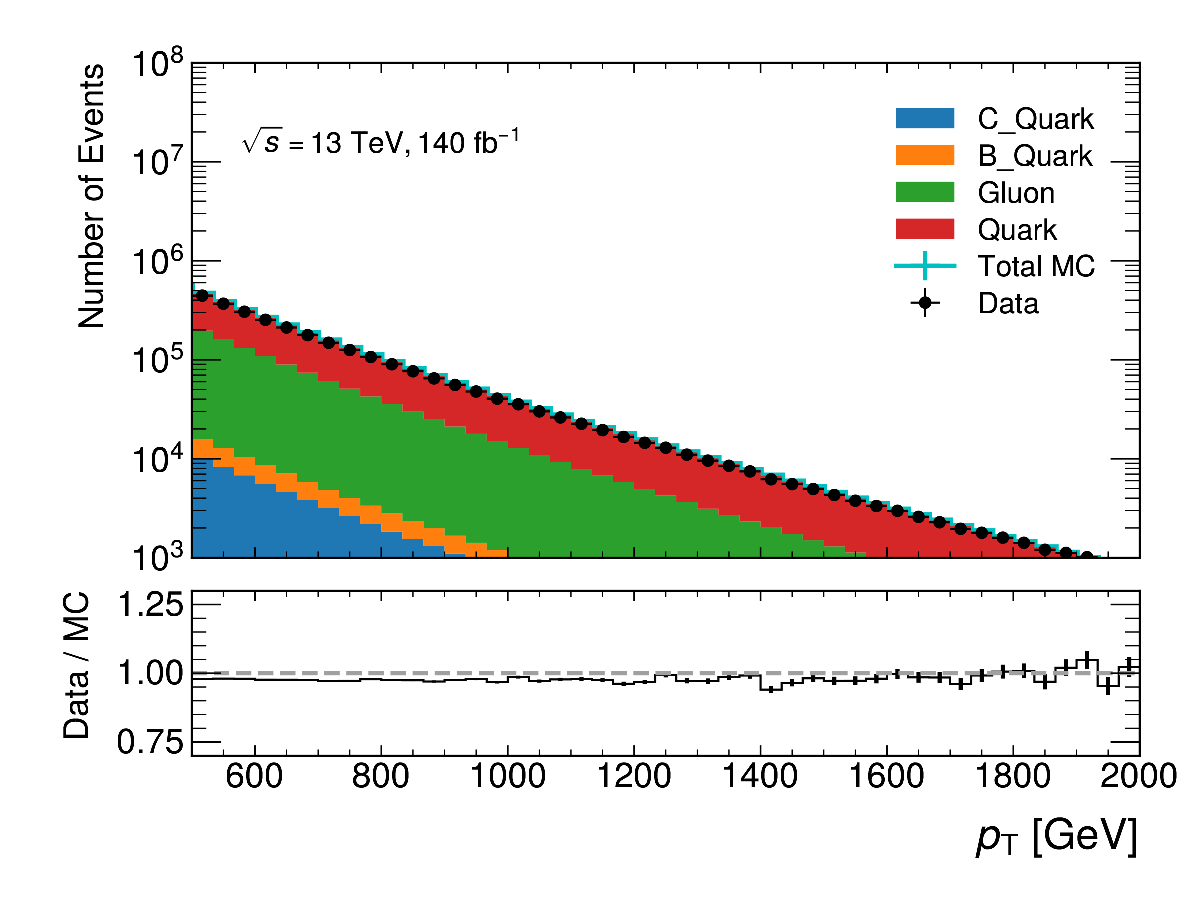
\includegraphics[width=0.48\textwidth]{fig/ADE/Pt_spectrum/none_event_weight/pt_MC16ADE_LeadingJet.pdf}} \quad
        \subfloat[subleading jet  ]{\label{fig:QG-2samplePtaa}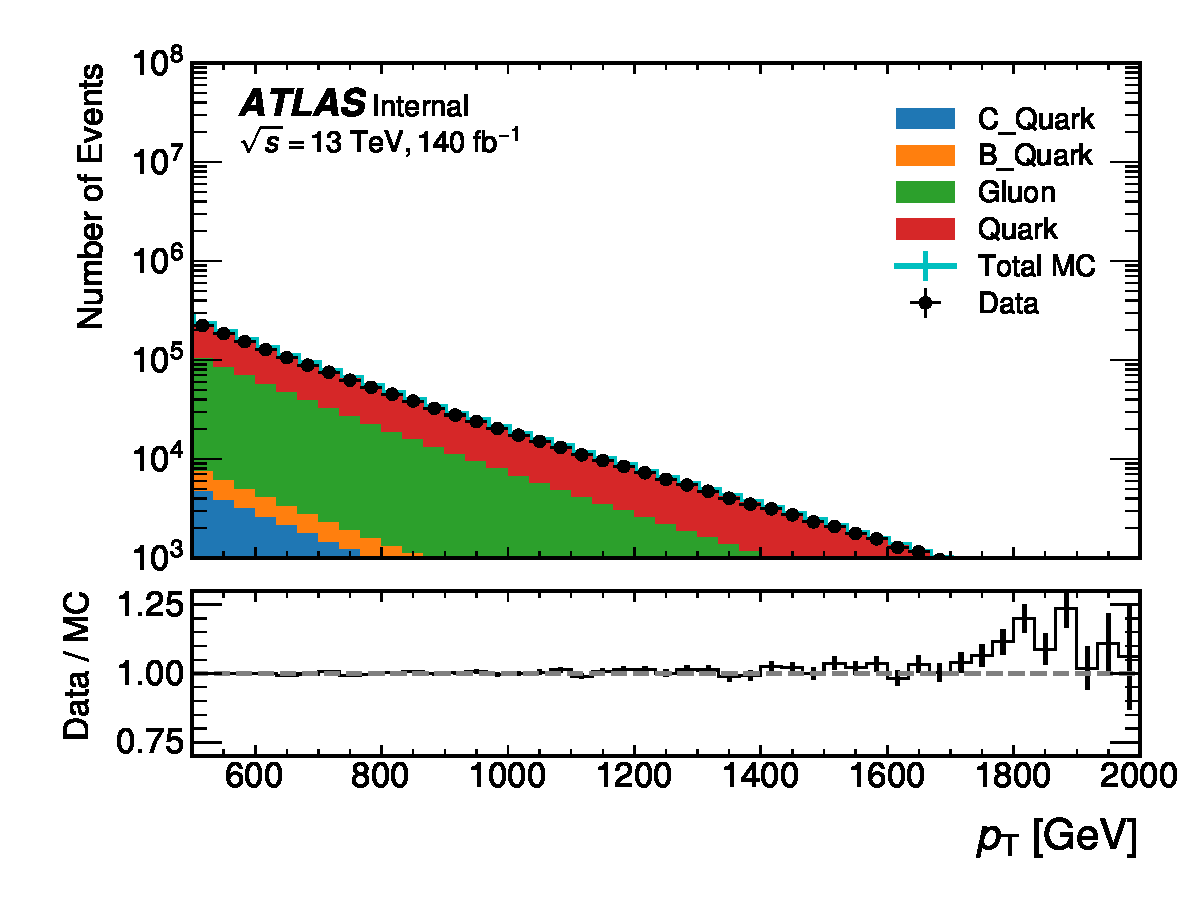
\includegraphics[width=0.48\textwidth]{fig/ADE/Pt_spectrum/none_event_weight/pt_MC16ADE_SubLeadingJet.pdf}} \quad
        \caption[]{
	  The \pt~distribution of the leading jets and sub-leading jets with \pythia samples for dijet event.
                \label{fig:QG-2samplePt}
        }
\end{figure}




